\begin{figure}[h]
\centering
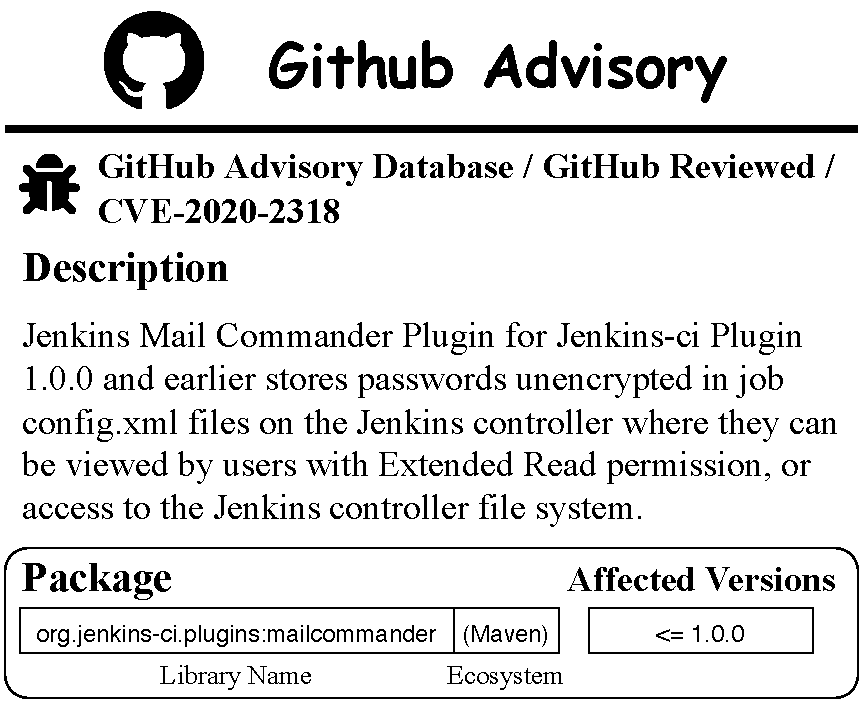
\includegraphics[width=1\linewidth]{figures/vulnerability-report.drawio.pdf}
\caption{GitHub Advisory Report for \href{https://github.com/advisories/GHSA-485q-v457-3p58}{CVE-2020-2318}}
\label{fig: case}
\vspace{-0.4cm}
\end{figure}

\section{Introduction}
\label{sec:intro}

One important task in security is to automatically extract the package names and versions affected by each security vulnerability. 
% With the increasing usage of third-party software packages, their security vulnerabilities pose great challenges to software and network systems.
A recent study~\cite{wang2020empirical} shows that 84\% third-party packages contain security vulnerabilities and 60\% of them are high-risk ones.
To mitigate the security risks, security practitioners maintain databases (e.g., NVD and GitHub Advisory) for each unique vulnerability (i.e., Common Weakness Enumeration or CVE). These databases contain reports with the vulnerability description, affected packages, and affected versions. For example, Figure~\ref{fig: case} shows the report of \href{https://github.com/advisories/GHSA-485q-v457-3p58}{CVE-2020-2318}. By linking the CVEs to the affected packages, developers can be aware of the vulnerable packages in their code and quickly apply patches/fixes; the affected packages also help with security knowledge management and task prioritization. Although developers can manually enter the affected packages when submitting CVEs, the entered information is often missing or incorrect~\cite{lightxml,viem}. While database maintainers also conduct manual reviews~\cite{githubReview}, automatic identification can accelerate the vulnerability lifecycle and reduce the manual costs, thus it is a critical task. 
%Figure~\ref{fig: case} shows an example report of one vulnerability, \href{https://github.com/advisories/GHSA-485q-v457-3p58}{CVE-2020-2318}.
%The vulnerability's affected packages include  \CodeIn{org.jenkins-ci.plugins:mailcommander} and its corresponding versions.
%The field of affected packages is specified by the developers who create this CVE. However, recent studies~\cite{lightxml,viem} show that in more than half of vulnerability reports, this field is missing or incorrect.
% \xueqing{can we say the package information is incorrect?}
% \tianyu{I think it's better not to mention incorrect, otherwise, our ground truth of labels might be challenged.}
%To alleviate this problem, human maintainers manually complete or validate the affected-package information in databases such as GitHub Advisory~\cite{githubReview}.
% \xueqing{replace reference inproceedings with misc}.
% \xueqing{Add citation to show that NVD or GitHub advisory packages are verified}.
%However, manual completion or validation requires high manual efforts~\cite{lightxml,vullibminer}, underscoring the need for automatic identification. 

% \xueqing{Explain how is smaller model used -> low accuracy -> leverage LLM's potential, LLM will keep improving-> if we use it the same way as smaller models, cost is high -> to leverage LLM wo high cost, propose the generative approach}

Several existing works have studied automatic affected package identification~\cite{fastxml, viem, lightxml, chronos, vullibminer}, however, it is challenging for them to achieve high accuracy because they fail to leverage large language models. Existing works typically rank/retrieve the package name from a list of pre-defined packages by computing the similarity between the vulnerability description and the package description. Since the time complexity of retrieval is linear to the size of the list (e.g., 435k Java packages), the cost of each model inference has to be kept quite low and only smaller models have been used, e.g., BERT and linear regression~\cite{fastxml,chronos,lightxml,vullibminer}. 

To leverage the extensive knowledge and semantic capabilities of LLMs, we propose a different strategy: \emph{generate rather than retrieve} the affected package. Our framework, \detector{}, is the first framework to directly generate the mentioned package name given the vulnerability description. Since generation requires the LLM inference to be invoked only once, our approach can easily scale to larger language models such as Llama-13B and Vicuna-13B on a single GPU server. 

% suffers from two related limitations on time cost and accuracy, respectively.  %lower accuracies while requiring a linear time cost with respect to the number of packages~\cite{chronos,vullibminer}. 
% First, existing work has linear time cost to the number of packages under consideration (e.g., 435k Java packages)~\cite{chronos,vullibminer}, so that the cost of each model inference has to be kept quite low. 
% Given a vulnerability description (Figure~\ref{fig: case}), existing work computes a similarity score between the vulnerability description and each package's text description from the ecosystem (e.g., PyPI, Maven), and then ranks all packages based on this score. As a result, the time cost for identifying each vulnerability = the number of candidate packages $\times$ the cost of each model inference (e.g., BERT). 
% Second, existing work suffers from low accuracy due to the adoption of a relatively small model. The first limitation causes the underlying model used for inference to be a relatively small model such as logistic regression and BERT~\cite{fastxml,chronos,lightxml,vullibminer}. 
% Second, regarding the time cost, given a vulnerability description (Figure~\ref{fig: case}), existing work requires to compute a similarity score between the vulnerability description and each package's text description from the ecosystem (e.g., PyPI, Maven), then they rank all package based on this score. As a result, the time cost for identifying each vulnerability = the number of candidate packages $\times$ the cost of each model inference (e.g., BERT). 

% To address the preceding limitations, in this paper, we propose the first work, a framework named \detector{}, to explore the use of a large language model (LLM) for identifying vulnerable packages, given the continuously and rapidly improved effectiveness brought by an LLM for various tasks. \detector{} uses an LLM to \emph{generate} the names of affected packages instead of ranking the names of packages under consideration. 
% Our rationale for not following the existing work's ranking approaches is that the number (denoted as $|\mathcal{P}|$) of packages under consideration (e.g., 435k Java packages) brings high cost to rank the similarity scores between a vulnerability and each package under consideration.
% In contrast, in order to identify vulnerable packages, the generative approach invokes the model inference only once, instead of $|\mathcal{P}|$ times.
% When using LLMs, we cannot directly adopt previous work's ranking approach, since the number of candidate packages (e.g., Java has 435k packages) and the inference cost of LLMs are both high. In contrast, the generative approach invokes the model inference only once.

%Specifically, \detector{} includes two techniques to address two main challenges of generating the names of affected packages.
Upon observing errors in the raw generation result of LLMs, we propose the following techniques for improving \detector{}'s accuracy. 
First, we conduct supervised fine-tuning (SFT), in-context learning, and retrieval-augmented generation (RAG) to enhance the domain knowledge of a LLM.
%as an LLM may lack the domain knowledge required to generate the name of the target package. During model inference, the vulnerability description as input fed to an LLM often does not contain the full information of the target package's name, and thus the LLM is required to infer the missing information based on  the domain knowledge. 
Second, we propose a novel local search technique to post-process the raw output for reducing hallucination, i.e., ensuring that the generated package name actually exists. Our local search algorithm is inspired by an empirical study of the incorrect raw outputs of ChatGPT. The study shows that most errors are partially correct, therefore we can create rules to match the incorrect part to the closest existing one given the correct part. Since the sub-level package information (e.g., \CodeIn{mailcommander} in Figure~\ref{fig: case}) is often more directly mentioned than the top-level package information (e.g., \CodeIn{org.jenkins-ci.plugins}), our local search algorithm first matches the suffix before the prefix. 

%Recent studies~\cite{vazquez2023javascript} show that an LLM may generate package names that do not exist. 
%Based on our empirical study of incorrect raw outputs of ChatGPT, we design our local search technique that matches the generation output with the closest package name among the names of the packages under consideration, and produces the matched package name as the final output.

% Second, to ensure the generated package exists, we propose a post-processing algorithm to match the generation output with the closest existing package name. Our algorithm design is based on an empirical study of the errors of the raw output of ChatGPT. 


% To address the preceding challenges, \detector{} includes two techniques. First, to enhance the domain knowledge of LLMs, we employ supervised fine-tuning, in-context learning, and retrieval-augmented generation (RAG). Second, to ensure the generated package exists, we propose a post-processing algorithm to match the generation output with the closest existing package name. Our algorithm design is based on an empirical study of the errors of the raw output of ChatGPT. 

% To improve the accuracy of the generation, \detector{} aims to address two issues with the generative approach. First, the LLM may lack the domain knowledge required to generate the target package. The reason is that the LLM's input vulnerability description often does not contain the full information of the package name, it thus requires the LLM to infer the missing information from the domain knowledge. Second, a previous study shows that the LLM may generate package names that do not exist. 

% To address the preceding issues, our approach includes two techniques. First, to enhance the domain knowledge of LLMs, we employ supervised fine-tuning, in-context learning, and retrieval-augmented generation (RAG). Second, to ensure the generated package exists, we propose a post-processing algorithm to match the generation output with the closest existing package name. Our algorithm design is based on an empirical study of the errors of the raw output of ChatGPT. 

% Existing work on automatic identification of vulnerable packages~\cite{fastxml, viem, lightxml, chronos, vullibminer} propose  ranking approaches\footnote{\xueqing{classification which can be seen as ranking approach}} that,  given the vulnerability description as the query, rank the most similar package name from an existing list of package names of the corresponding ecosystem (e.g., PyPI, Maven). Since a ranking approach requires one to compute the description's similarity with each package, the time cost is typically large, e.g., Java has 435k packages. To the best of our knowledge, most existing approaches focus on relatively smaller models such as non-neural-network models~\cite{fastxml}, logistic regression~\cite{zestxml,chronos}, or BERT~\cite{lightxml,vullibminer}. Without leveraging larger models, they typically suffer from low accuracies. 


% However, these approaches face the scalability problem due to the large number of third-party packages (e.g., more than 500 thousand).
% Now that it is time-consuming to correlate each package with a given vulnerability description, a large portion of existing approaches use only lightweight models, such as FastXML~\cite{fastxml} and ZestXML~\cite{chronos} to rank these packages, thus leading to low accuracies.
% Although other approaches~\cite{vullibminer} adopt reranking models after the lightweight ranking model, the number of candidate packages (e.g., 512) still leads to a heavy burden of time and computation resources, especially when adopting large language models (LLMs).

% Specifically, both of these approaches are limited to their training set~\cite{fernandez2011semantically}.
% Thus, they are ineffective in identifying unseen vulnerable libraries during training.

% To address the low accuracy issue, in this paper, we propose to first leverage large language models (i.e., 7B models and larger) for vulnerable package identification. Given the description, our approach will \emph{generate}, rather than rank the package names. As a result, our approach can scale to larger models since this approach requires invoking the model inference only once. However, it is unclear whether the generative approach is effective for this task. On the one hand, the description often does not include the full information about the package name (Section~\ref{sec: empirical_study}); on the other hand, the task requires the generated package name to exactly match the ground truth and previous work finds this to be challenging for LLMs~\cite{liu2023codegen4libs}. To understand the potential of the generative approach, we conduct a pilot study on the errors made by ChatGPT raw output for this task. The study shows that ChatGPT raw output has a reasonable accuracy; however, for some vulnerabilities, ChatGPT lacks the domain knowledge for generation; for other vulnerabilities, the generated package names do not exist. 
%Based on the study results,
% \xueqing{I named the task vulnerable package identification, please check}.
% Nevertheless, text generation suffers from challenges such as hallucination~\cite{ji2023survey} which may affect the accuracy. To understand the feasibility of the generative approach, we first conduct a pilot study on how ChatGPT output for this task. We observe that with 42\% probability, the raw output correctly matches the ground truth. Among the incorrect outputs, 22.4\% can be fixed by matching the output with the closest existing package.
% \xueqing{Check if this statement is true}.
%(3) Among the rest incorrect names, ChatGPT captures incorrect keywords or fails to capture keywords from vulnerability descriptions due to its lack of knowledge.
% From the results of the preceding empirical study, we categorize two main challenges that lead to incorrectly generated names.
% First, LLMs lack sufficient domain knowledge of these affected libraries.
% For example, a Java package's name consists of both group IDs and artifact IDs while the group ID might be neglected in a vulnerability description.
% Therefore, LLMs need to generate the correct group ID based on their domain knowledge.
% Second, LLMs might output non-existing package names.
% Note that LLMs generate the names of affected packages from only vulnerability descriptions, so the output names might have more/fewer tokens, e.g., \CodeIn{core} or \CodeIn{framework}, which are widely used in the names of Java packages.



% To address the preceding challenges, we design three techniques to address the preceding challenges.
% First, we design a retrieval augmented generation (RAG) technique that provides domain knowledge into the inputs of LLMs before generation.
% Specifically, we add the names of affected libraries generated by IR approaches as they might be similar to the targeted library names.
% Second, we design a constrained decoding algorithm during generation.
% We collect package names from ecosystems of each programming language and require the output of LLMs to include at least one of them, thus avoiding non-existing package names.
% This technique modifies the decoding layer of LLMs and can be applied to only open-source LLMs.
% Third, we design a local search algorithm after generation.
% It directly searches the closest package name for each generated name, thus also avoiding non-existing package names.
% This technique is non-intrinsic and can be applied to both commercial and open-source LLMs.


We evaluate \detector{} on four vulnerability ecosystems: Java, JS, Python and Go. Our evaluation attains three main findings. First, we observe that the accuracy of \detector{} (0.806) significantly outperforms existing ranking approaches using smaller models~\cite{fastxml,lightxml,chronos,vullibminer} (0.721) and the computational time costs are comparable. 
%In particular, \detector{} using Vicuna-13B outperforms the larger ChatGPT and GPT-4 models by employing supervised fine-tuning (SFT). 
Second, our ablation studies show that SFT, RAG, and local search all help improve the accuracy of \detector{} and SFT contributes to the most improvement. In particular, the fine-tuned open-source Vicuna-13B outperforms the unfine-tuned commercial ChatGPT and GPT-4 models. Our local search algorithm can significantly reduce the hallucination in the original LLM output, and it is especially helpful for longer package names such as Java and Go. Third, \detector{} provides high value to security practice: at the time of the writing, we have submitted 60 pairs of <vulnerability, affected package> to GitHub Advisory (25 Java, 14 JS, 11 Python, 10 Go) and 34 of them have been accepted and merged.
% Additionally, the source code and dataset of \detector{} can be found in \url{https://github.com/q5438722/VulLibGen}.
% To examine \detector{}'s performance in the real-world setting, we further randomly sample a subset of the vulnerability descriptions in Java and JS, use \detector{} to generate the package names, and submit the generated names to GitHub Advisory. Among the 28 submitted <vulnerability, affected package> pairs, 22 are accepted and merged. This result highlights the real-world performance of \detector{} in automatically generating the names of affected packages. 

% We evaluate \detector{} using four state-of-the-art/practice (SOTA) approaches (FastXML~\cite{fastxml}, LightXML~\cite{lightxml}, Chronos~\cite{chronos}, and VulLibMiner~\cite{vullibminer}) that identify vulnerable libraries on the dataset of GitHub Advisory.
% Our evaluation results show that:
% (1) \detector{} is highly effective, achieving an accuracy of 0.806 while the best of SOTA approaches achieves only 0.669.
% (2) Our RAG technique and local search algorithm can boost the effectiveness of \detector{} by 8.9\% and 3.0\% on average, respectively.
% (3) \detector{} achieves better trade-offs between efficiency and accuracy than both existing and future ranking approaches.
% (4) \detector{} brings high value to security practice. 
% We have submitted 28 pairs of <vulnerability, affected package> to GitHub advisory, and 22 of them have been accepted and merged.
% We submit 25 vulnerabilities' affected libraries to GitHub advisory and 18 of them are accepted and merged.
% (5) Although fine-tuned open-source LLMs achieve similar effectiveness with ChatGPT/GPT4, they might face the limitation of overfitting, which can be alleviated by larger open-source LLMs.\tianyu{is it necessary to keep (5)?}



% Existing approaches~\cite{fastxml, viem, lightxml, chronos, vullibminer} model this task as an information retrieval (IR) task or a classification task.
% For example, they take the description field \CodeIn{``Jenkins Mail Commander Plugin for Jenkins-ci Plugin 1.0.0 and earlier stores passwords unencryted $\dots$''} as inputs and their targeted outputs, are the field of affected libraries, e.g., \CodeIn{maven:org.jenkins-ci.plugins:mailcommander}.
% However, these approaches face the scalability problem as it is unavoidable for IR/classification approaches.
% Specifically, both of these approaches are limited to their training set~\cite{fernandez2011semantically}.
% Thus, they are ineffective in identifying unseen vulnerable libraries during training.

% To address the scalability problem, in this paper, we propose to model this task as a generation task, thus utilizing the tremendous capabilities of Large Language Models (LLMs) in comprehending vulnerability descriptions.
% Here, we collect the dataset from the reviewed reports in GitHub Advisory.
% The affected libraries in each report are submitted by library developers and users, and they are manually validated by the maintainers of GitHub Advisory.
% Therefore, the ground truth of this dataset is reliable.
% Specifically, the number of Java, JavaScript, Python, and Go vulnerabilities are 4308, 3193, 2237, and 1351, respectively.


% Before employing LLMs for this task, we conduct an empirical study on the results when directly querying ChatGPT, revealing two main categories of challenges faced by LLMs.
% First, LLMs lack sufficient domain knowledge of these affected libraries.
% For example, in CVE-2022-24197, the affected library is \CodeIn{maven:com.itextpdf:itext7-core} while its description only mentions the affected library's artifact ID \CodeIn{itext7-core}, and its group ID \CodeIn{com.itextpdf} is neglected. 
% This group ID can be complemented based on the domain knowledge that only \CodeIn{itext7-core} corresponds to only one group ID \CodeIn{com.itextpdf}.
% Second, LLMs might output non-existing library names.
% For example, in CVE-2020-2167, the affected library is \CodeIn{maven:com.openshift.jenkins:openshift-pipeline} while LLMs might change the group ID into \CodeIn{com.openshift.jenkins}, which is not an existing library.
% % \tianyu{I also consider the reason that there might exist vulnerabilities whose descriptions are incomplete. (in the following comments in the source code)
% % However, this reason might be similar to 'lack of domain knowledge'}
% % First, the information in vulnerability reports might be incomplete. 
% % For example, in CVE-2017-1000406, the affected library is \CodeIn{maven:org.opendaylight.integration:distribution-karaf} while token \CodeIn{distribution} does not occur in its description.
% % Thus, even human experts cannot identify the correct names of affected libraries.


% To address the preceding challenges, we design two categories of techniques to address the preceding challenges.
% First, we design a retrieval augmented generation (RAG) technique that provides domain knowledge into the inputs of LLMs. 
% Specifically, we add the names of affected libraries generated by IR approaches as they might be similar to the targeted library names.
% Second, we design a constrained decoding algorithm and a local search algorithm to reduce non-existing outputs.
% Specifically, the constrained decoding algorithm is more effective while the local search algorithm is non-intrinsic and can be applied in commercial LLMs, e.g., ChatGPT/GPT4.
% Both algorithms utilize the database of all library names (e.g., those in Maven or Pypi) to ensure that the output of \detector{} is an existing library name.


% We evaluate \detector{} using three state-of-the-art/practice (SOTA) approaches (LightXML~\cite{lightxml}, Chronos~\cite{chronos}, and VulLibMiner~\cite{vullibminer}) that identify vulnerable libraries on the dataset of GitHub Advisory.
% Our evaluation results show that:
% (1) \detector{} is highly effective, achieving an accuracy of 0.80 while the best of SOTA approaches achieves only 0.669.
% (2) Our RAG technique can boost the effectiveness of both ChatGPT/GPT4 and open-source LLMs by at least 12\%.
% (3) Both our constrained decoding and local search algorithms can effectively reduce incorrect/non-existing outputs by at least 5.4\%.
% (4) \detector{} brings high value to security practice. We submit 25 vulnerabilities' affected libraries to GitHub advisory and 18 of them are accepted and merged.
% (5) Although fine-tuned open-source LLMs achieve similar effectiveness with ChatGPT/GPT4, they might face the limitation of overfitting, which can be alleviated by larger open-source LLMs.


% 一个建议的intro提纲:
% 1. CVE问题的重要性(为什么需要自动预测,可以帮助及时修补?)
% 2.当前解决方案的不足(scalability)
% 3.我们提出用generation来解决scalability问题,介绍一下GitHub advisory数据集以及为什么ground truth是准确的,3.但是generation存在挑战:一个是有的example input信息不全(所以即使human expert也很难做到100%),一个是llm缺乏domain knowledge 
% 4.做一个empirical study发现input信息不全的现象只占少数。同时针对以上挑战,设计了几个方法:fine tuning,rag,constrained decoding,post processing,讨论一下它们为什么有可能解决generation的挑战。
% 5. 总结实验结果,讨论可能存在的limitation,比如fine tuning可能存在overfitting,future work如何弥补这些limitation


% To avoid potential risks posed by vulnerabilities in third-party libraries, security researchers maintain databases containing vulnerability reports, e.g., the National Vulnerability Database (NVD)~\cite{nvd}. 
% A vulnerability report in NVD includes a vulnerability's identification number in the entry of Common Vulnerability Enumeration (CVE), its description, and the name list of libraries affected by the vulnerability  (a.k.a. vulnerable libraries).
% Application developers can identify vulnerable libraries by directly querying each description and CPE entry with the name of each used library. 
% However, recent studies on about 200,000 vulnerability reports in NVD show that 53.3\% of the vulnerability reports in NVD do not mention any affected libraries~\cite{lightxml} and 59.82\% of the included vulnerable libraries are incomplete or incorrect~\cite{viem}.


% To address the preceding issue, existing approaches~\cite{viem, anwar2021cleaning, jo2022vulcan, kuehn2021ovana, fastxml, lightxml, chronos, vullibminer} fall into three main categories.
% First, named-entity-recognition (NER) approaches~\cite{viem, anwar2021cleaning, jo2022vulcan, kuehn2021ovana} use NER models to extract the mentioned library entities from vulnerability descriptions, and then match these entities with a dictionary of library names.
% Second, extreme multi-label learning (XML) approaches~\cite{fastxml, lightxml, chronos} use deep-learning classification models to assign a set of labels (i.e., vulnerable libraries) to a given vulnerability by training on labeled datasets.
% Third, entity-linking approaches~\cite{vullibminer} take library descriptions as inputs besides the description of a given vulnerability, thus achieving higher accuracy than NER and XML approaches.

% Although existing approaches make efforts to identify vulnerable libraries, they still suffer from highly inaccurate results.
% Existing NER and XML approaches cannot distinguish vulnerable libraries with similar names, such as ``org.jenkins-ci.plugins:mailer'' and ``org.jenkins-ci.plugins:mailcommander''.
% However, these libraries are not affected together by one vulnerability due to their different functionalities and scopes.
% Existing entity-linking approaches use TF-IDF techniques to reduce the number of libraries for comparison, and yet suffer from false negatives (i.e., some vulnerable libraries are missed) and thus low accuracy.
% Considering the large number of collected libraries (e.g., 310,844 in Maven) for comparison compared, this step cannot be avoided; otherwise, it might cost them two years to identify all vulnerable libraries~\cite{vullibminer}.




% To overcome the preceding limitations, we propose \detector{}, the first generative approach to generate the affected libraries of a given vulnerability.
% \detector{} is effective to generate the name list of vulnerable libraries (out of all the existing libraries) by utilizing the recent enormous advances in Large Language Models (LLMs) with two stages of fine-tuning.
% The rationale behind this step is that LLMs can correlate the input vulnerability description to vulnerable libraries based on their prior knowledge of these libraries, e.g., their functionalities, usages, and even history issues.
% With prior knowledge, \detector{} avoids the high cost of correlating one vulnerability description with each library.
% Specifically, we conduct unsupervised fine-tuning on maven~\cite{maven} corpus to fine-tune raw LLaMa models to activate their prior knowledge of Java libraries.
% The input of this stage is one library's description, and its targeted output is its library name.
% Then, we conduct supervised fine-tuning on labeled datasets to enhance the ability to identify vulnerable libraries.
% The input of this stage is a vulnerability description and its targeted output is a name list of vulnerable libraries affected by this vulnerability.

% Since we use fine-tuned LLMs to generate the affected library names of a given vulnerability, there are two main challenges that decrease LLMs' effectiveness.
% First, LLMs face the difficulty of low accuracy when identifying zero-shot libraries because they have no prior knowledge of how these libraries are affected by vulnerabilities.
% Similar to XML approaches, LLMs tend to output incorrect libraries that have already been affected by other vulnerabilities during training and fine-tuning.
% Second, LLMs face hallucinations, i.e., generating plausible-looking library names that are non-existing.
% For example, they might mix up two similar library names and lack part of the library names.



% To address the preceding challenges, we design two specialized techniques during supervised fine-tuning to improve the effectiveness by addressing the preceding challenges.
% To help identify zero-shot libraries, we design an input augmentation technique, which feeds the names of vulnerable libraries (a.k.a., recommended libraries) identified by the SOTA approach~\cite{vullibminer} to \detector{} as input.
% This technique provides examples of libraries whose functionalities are likely to be affected by a given vulnerability.
% Thus, \detector{} can generate library names from those with similar functionalities instead of all libraries when \detector{} has no prior knowledge of how these zero-shot libraries are affected by vulnerabilities.
% To address \detector{}'s hallucinations, we design our post-processing technique based on the Levenshtein distance~\cite{levenshtein} to obtain existing Java library names from the response of LLMs.
% We find that \detector{} can generate the components of the targeted library names (i.e., the targeted functionalities and scopes), and make mistakes when jointing these components of library names, thus leading to hallucinations.
% Therefore, hallucination library names are close to the targeted names of vulnerable libraries, and their closest library names tend to be the targeted names.


% We evaluate \detector{} using three state-of-the-art/practice approaches (LightXML~\cite{lightxml}, Chronos~\cite{chronos}, and VulLibMiner~\cite{vullibminer}) that identify vulnerable libraries on an open-source dataset (VulLib)~\cite{vullib}.
% Our evaluation results show a number of findings to demonstrate our \detector{} approach’s effectiveness and efficiency.
% Given the ground truth score of 0.840, \detector{} effectively achieves the F1@1 score of 0.626 while the state-of-the-art/practice (SOTA) approaches achieve only 0.561.
% Specifically, the post-processing technique helps \detector{} achieve an average improvement of F1@1 by 9.3\%, and the input augmentation technique helps \detector{} achieve an average improvement of F1@1 by 39\% in identifying zero-shot libraries.
% Additionally, \detector{} is highly efficient, identifying one vulnerability in less than 6 seconds.


% In summary, this paper makes the following main contributions:
% \begin{itemize}
% \item  We propose, \detector{}, the first generative approach for identifying vulnerable libraries via Large Language Models.
% \item  We design an input augmentation technique and a post-processing technique to help identify zero-shot libraries and help address hallucinations.
% \item  We conduct a comprehensive evaluation demonstrating the effectiveness and efficiency of \detector{}, increasing the F1@1 of 0.626 while the state-of-the-art/practice (SOTA) approaches achieve only 0.561.
% \end{itemize}

